%% whole_genome_comparisons.tex
%% Author: Leighton Pritchard
%% Copyright: James Hutton Institute
%% Whole genome comparisons

%
\begin{frame}
  \frametitle{Whole genome comparisons}
  \Large{
    \textcolor{olive}{
      \textbf{
      Comparisons of one whole or draft genome with another \\
      ($\ldots$or many others)
      }
    }
  }
\end{frame}

%
\begin{frame}
  \frametitle{Whole genome comparisons}
  Minimum requirement: \textbf{two genomes} \\
  \begin{itemize}
    \item \textcolor{hutton_green}{Reference Genome}
    \item \textcolor{hutton_blue}{Comparator Genome}
  \end{itemize}
  The experiment produces a comparative result \textcolor{hutton_purple}{\textit{that is dependent on the choice of genomes}}.
\end{frame}

%
\begin{frame}
  \frametitle{Whole genome comparisons}
  Experimental methods mostly involve direct or indirect DNA hybridisation \\
  \begin{itemize}
    \item \textcolor{hutton_green}{DNA-DNA hybridisation (DDH)}
    \item \textcolor{hutton_blue}{Comparative Genomic Hybridisation (CGH)}
    \item \textcolor{hutton_purple}{Array Comparative Genomic Hybridisation (aCGH)}    
  \end{itemize}
\end{frame}

%
\begin{frame}
  \frametitle{Whole genome comparisons}
  Analogously, \textit{in silico} methods mostly involve sequence alignment \\
  \begin{itemize}
    \item \textcolor{hutton_green}{Average Nucleotide Identity (ANI)}
    \item \textcolor{hutton_blue}{Pairwise genome alignment}
    \item \textcolor{hutton_purple}{Multiple genome alignment}    
  \end{itemize}
\end{frame}

%
\begin{frame}
  \frametitle{DNA-DNA hybridisation (DDH)
  \footnote{\tiny{\href{http://dx.doi.org/10.1016/S0168-6445(00)00040-1
}{Morell\'{o}-Mora \& Amann (2011) \textit{FEMS Microbiol. Rev.} doi:10.1016/S0168-6445(00)00040-1
}}}
  }
  Several similar methods based on the same principle
  \begin{columns}[T] 
    \column{.4\textwidth} 
      \begin{itemize}
        \item \textcolor{hutton_green}{Denature gDNA mixture for organisms $A$, $B$}
        \item \textcolor{hutton_blue}{Allow gDNA to anneal; hybrids result}
      \end{itemize}
    \column{.6\textwidth}
      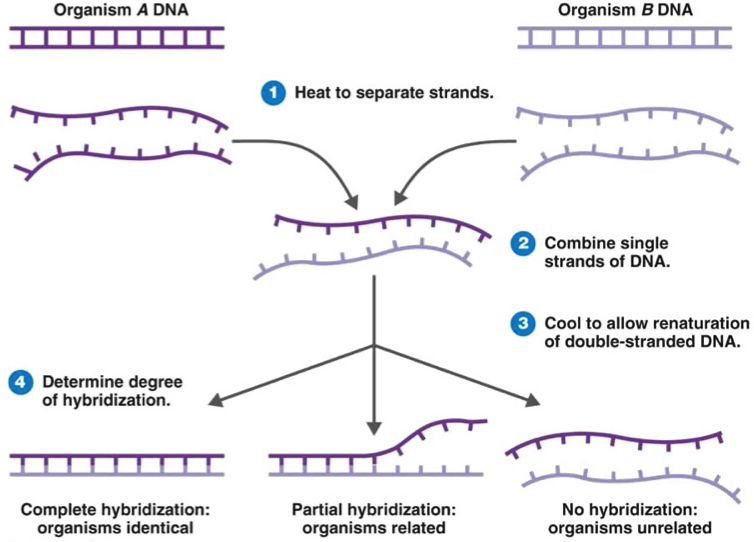
\includegraphics[width=\textwidth]{images/dna-dna_hyb}
  \end{columns}    
  \textcolor{hutton_green}{Reassociation of gDNA $\approx$ sequence similarity}
\end{frame}

%
\begin{frame}
  \frametitle{Average Nucleotide Identity (ANI)
  \footnote{\tiny{\href{http://dx.doi.org/10.1099/ijs.0.64483-0
}{Goris \textit{et al.} (2007) \textit{Int. J. System. Evol. Biol.} doi:10.1099/ijs.0.64483-0
}}}
  }
  Introduced as an \textit{in silico} substitute for DDH in 2007:
  \begin{columns}[T] 
    \column{.6\textwidth} 
      \begin{itemize}
        \item \textcolor{hutton_green}{70\% identity (DDH) = "gold standard" prokaryotic species boundary}
        \item \textcolor{hutton_blue}{70\% identity (DDH) $\approx$ 95\% identity (ANI)}
      \end{itemize}
    \column{.4\textwidth}
      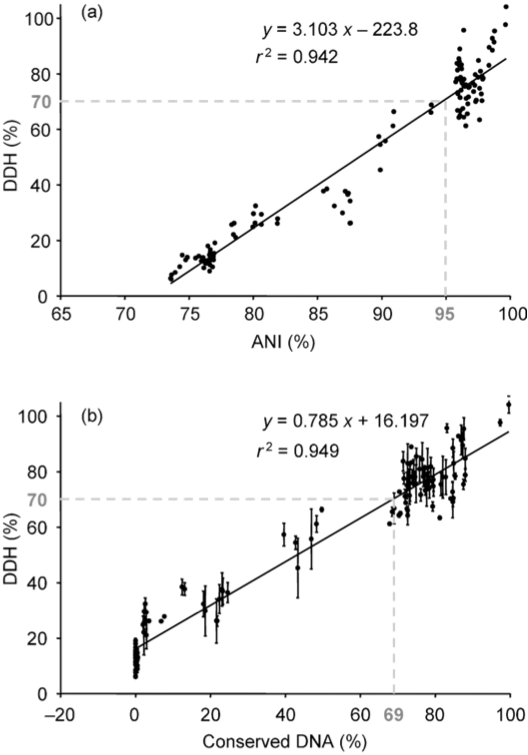
\includegraphics[width=\textwidth]{images/ani_ddh_equiv}
  \end{columns}    
\end{frame}

%
\begin{frame}
  \frametitle{Average Nucleotide Identity (ANI)
  \footnote{\tiny{\href{http://dx.doi.org/10.1073/pnas.0906412106
}{Richter \& Rossell\'{o}-M\'{o}ra \textit{et al.} (2009) \textit{Proc. Natl. Acad. Sci. USA} doi:10.1073/pnas.0906412106
}}}
  }
  ANIm and TETRA variants introduced in 2009:
  \begin{columns}[T] 
    \column{.5\textwidth} 
      \textcolor{RawSienna}{ANIm}
      \begin{enumerate}
        \item \textcolor{hutton_green}{Align sequences with NUCmer}
        \item \textcolor{hutton_purple}{ANI = mean identity of matches}
      \end{enumerate}
    \column{.5\textwidth}
      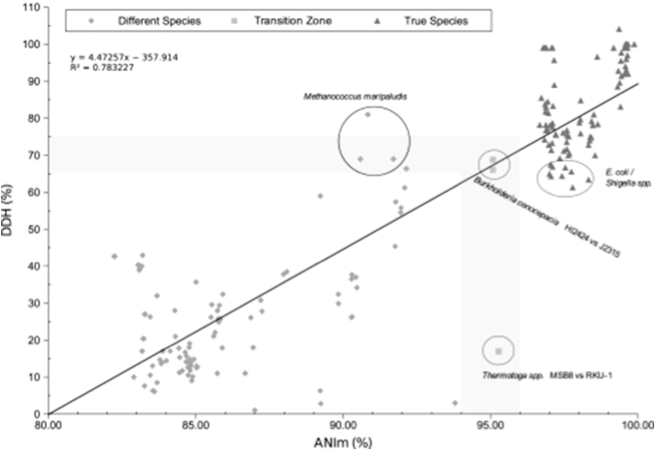
\includegraphics[width=\textwidth]{images/anim_ddh_equiv}
  \end{columns}    
  \textcolor{RawSienna}{TETRA} (a bulk measure!)
  \begin{enumerate}
    \item \textcolor{hutton_green}{Calculate 4-mer frequencies}
    \item \textcolor{hutton_blue}{Determine Z-score for 4-mer deviation from expected value, given \%GC content}
    \item \textcolor{hutton_purple}{TETRA = Pearson correlation coefficient of Z-scores}
  \end{enumerate}
\end{frame}

% ANIm in practice
\begin{frame}
  \frametitle{ANI in practice
    \footnote{\tiny{\href{http://dx.doi.org/10.1099/ijs.0.052944-0}{van der Wolf \textit{et al}. (2014) \textit{Int. J. Syst. Evol. Micr.} \textbf{64}:768-774 doi:10.1099/ijs.0.052944-0
    }}}
    \footnote{\tiny{\href{http://dx.doi.org/10.1039/C5AY02550H}{Pritchard \textit{et al}. (2016) \textit{Anal. Methods} \textbf{8}:12-24 doi:10.1039/C5AY02550H
    }}}
    }
  \begin{columns}[T]
    \begin{column}{5cm}
    \textit{Dickeya} species structure \\
      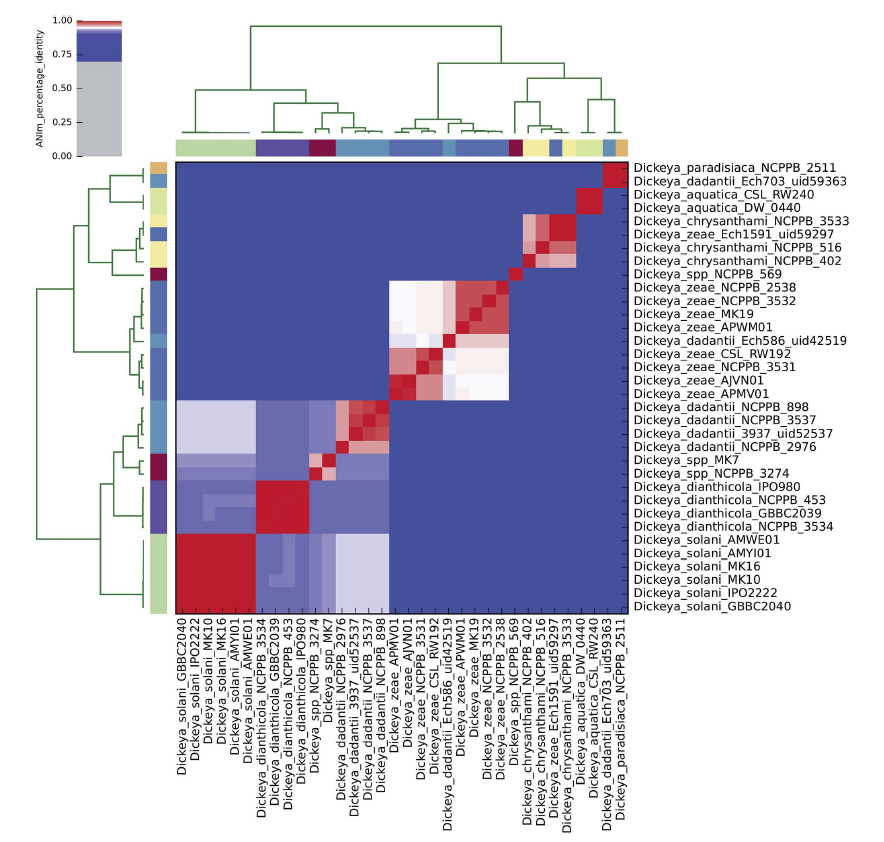
\includegraphics[width=\textwidth]{images/ANIm_dickeya}
    \end{column}
    \begin{column}{5cm}
    \textit{Pectobacterium} species structure:\\
      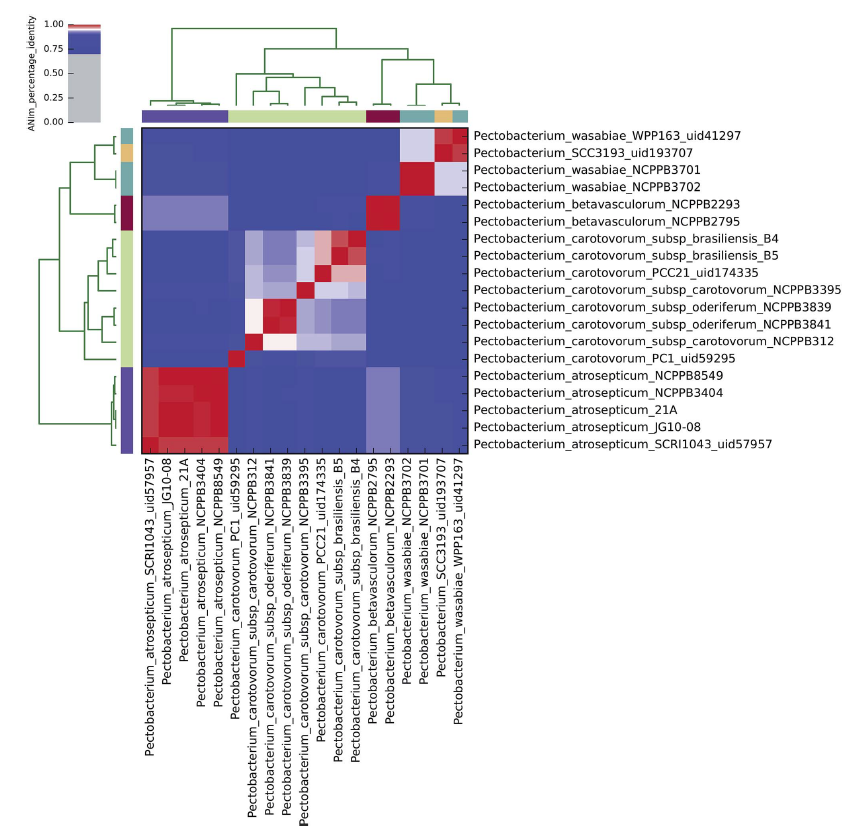
\includegraphics[width=\textwidth]{images/ANIm_pecto}
    \end{column}
  \end{columns}       
\end{frame}

%
\begin{frame}
  \frametitle{Pairwise genome alignments}
  \textcolor{olive}{Pairwise comparisons require alignment of similar regions.}
  \begin{center}
    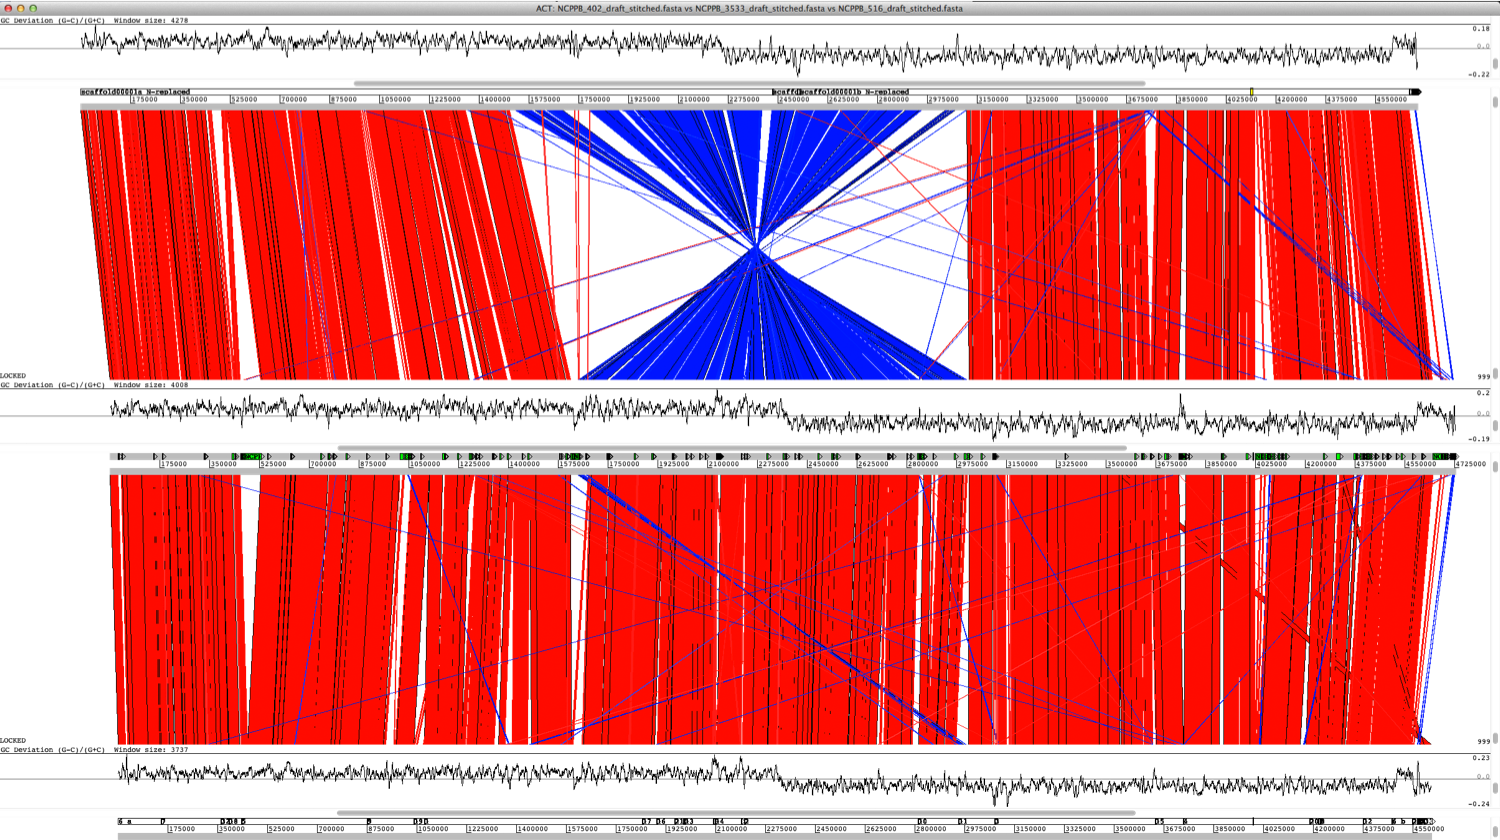
\includegraphics[width=\textwidth]{images/pairwise_genome_alignment}
  \end{center}  
\end{frame}

%
\begin{frame}
  \frametitle{Synteny and Collinearity}
  \textcolor{olive}{Genome rearrangements may occur post-speciation} \\
  Sequence similarity, and order of similar regions, may be conserved
  \begin{center}
    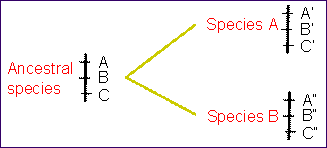
\includegraphics[width=0.5\textwidth]{images/collinear}    
    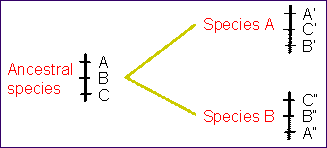
\includegraphics[width=0.5\textwidth]{images/synteny}
  \end{center}    
  \begin{itemize}
    \item \textcolor{hutton_blue}{\textit{collinear}} conserved elements lie in the same linear sequence
    \item \textcolor{hutton_purple}{\textit{syntenous} (or \textit{syntenic})} elements:
    \begin{itemize}
      \item (\textit{orig.}) lie on the same chromosome
      \item (\textit{mod.}) are collinear
    \end{itemize}
  \end{itemize}
  Evolutionary constraint (e.g. indicated by synteny) may indicate a functional constraint
\end{frame}

%
\begin{frame}
  \frametitle{Alignment algorithms/programs}
  \textcolor{hutton_green}{I assume you're familiar with BLAST} \\
  \textcolor{RawSienna}{Na\"{i}ve alignment algorithms are not appropriate}:
  \begin{itemize}
    \item Needleman-Wunsch: optimal global alignment
    \item Smith-Waterman: optimal local alignment
  \end{itemize}
  \textcolor{hutton_blue}{Cannot handle rearrangement} \\
  \textcolor{hutton_purple}{Computationally expensive}  
\end{frame}

%
\begin{frame}
  \frametitle{Alignment algorithms/programs}
  \textcolor{hutton_green}{Many whole-genome alignment algorithms proposed} \\
  Handle genome-scale evolutionary processes, scalable \\~\\
  \begin{itemize}
    \item \href{http://www.bx.psu.edu/~rsharris/lastz/}{LASTZ (http://www.bx.psu.edu/$\sim$rsharris/lastz/)}
    \item \href{http://genome.ucsc.edu/goldenPath/help/blatSpec.html}{\textcolor{hutton_blue}{\textbf{BLAT} (http://genome.ucsc.edu/goldenPath)}}
    \item \href{http://mugsy.sourceforge.net/}{Mugsy (http://mugsy.sourceforge.net/)}
    \item \href{http://www.ncbi.nlm.nih.gov/blast/html/megablast.html}{\textcolor{red}{\textbf{megaBLAST} (http://www.ncbi.nlm.nih.gov/blast/)}}
    \item \href{http://mummer.sourceforge.net/}{\textcolor{red}{\textbf{MUMmer} (http://mummer.sourceforge.net/)}}
    \item \href{http://lagan.stanford.edu/lagan_web/index.shtml}{{\textcolor{hutton_blue}{LAGAN (http://lagan.stanford.edu/lagan\_web/index.shtml)}}}
    \item WABA, etc?
  \end{itemize}
\end{frame}

%
\begin{frame}
  \frametitle{megaBLAST
  \footnote{\tiny{Zhang \textit{et al.} (2000) \textit{J. Comp. Biol.} \textbf{7}(1-2): 203-214
}}
  \footnote{\tiny{Korf \textit{et al.} (2003) \textit{BLAST} O'Reilly \& Associates, Sebastopol, CA
}}
  }
  Optimised for:
  \begin{itemize}
    \item \textcolor{hutton_green}{speed and genome-level searching}
    \item \textcolor{hutton_blue}{queries on large sequence sets}: "query-packing"
    \item \textcolor{hutton_purple}{long alignments of very similar sequences} (\url{dc-megablast} for divergent sequences)
  \end{itemize}
  Uses Zhang et al. greedy algorithm, \textbf{not BLAST algorithm} \\~\\
  \textcolor{RawSienna}{BLASTN+ defaults to megaBLAST algorithm} \\
  (see \href{http://www.ncbi.nlm.nih.gov/blast/Why.shtml}{http://www.ncbi.nlm.nih.gov/blast/Why.shtml})
\end{frame}

%
\begin{frame}
  \frametitle{MUMmer
  \footnote{\tiny{\href{http://dx.doi.org/10.1186/gb-2004-5-2-r12
}{Kurtz \textit{et al.} (2004) \textit{Genome Biol.} doi:10.1186/gb-2004-5-2-r12
}}}
  }
  Conceptually completely different to BLAST/BLAT/megaBLAST \\
  \textcolor{RawSienna}{Uses \textit{suffix trees} for pattern matching}
  \begin{itemize}
    \item \textcolor{hutton_green}{Finds maximal exact matches}
    \item \textcolor{hutton_blue}{Memory use depends only on reference sequence size}
  \end{itemize}
  \begin{columns}[T] 
    \column{.5\textwidth} 
      \textcolor{hutton_purple}{Suffix Tree:}
      \begin{itemize}
        \item Constructed and searched in $O(n)$ time
        \item Useful algorithms are nontrivial
        \item \url{BANANA$}
      \end{itemize}
    \column{.5\textwidth}
      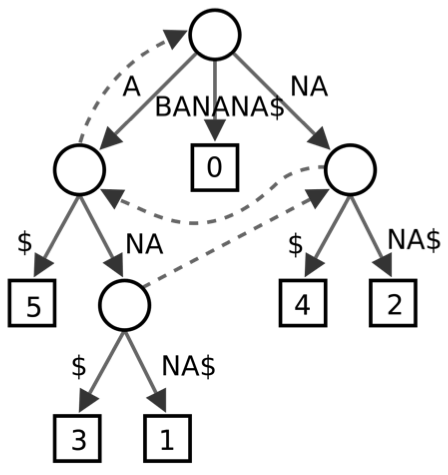
\includegraphics[width=0.75\textwidth]{images/suffix_tree}
  \end{columns}    
\end{frame}

%
\begin{frame}
  \frametitle{Pairwise genome alignments}
  \textcolor{hutton_green}{Which genomes should you align (or not bother with)?} \\
  \textcolor{RawSienna}{For reasonable analysis, genomes should}:
  \begin{itemize}
    \item derive from a sufficiently \textcolor{red}{recent} common ancestor, so that \textcolor{hutton_purple}{homologous regions can be identified}
    \item derive from a sufficiently \textcolor{red}{distant} common ancestor, so that \textcolor{hutton_purple}{biologically meaningful changes are likely to be found}
  \end{itemize}
\end{frame}

% Vibrio mimicus
\begin{frame}
  \frametitle{\textit{Vibrio mimicus} 
  \footnote{\tiny{\href{http://dx.doi.org/10.1073/pnas.1013825107}{Hasan \textit{et al}. (2010) \textit{Proc. Natl. Acad. Sci. USA} \textbf{107}:21134-21139 doi:10.1073/pnas.1013825107}}}
  }
  Chromosome C-II carries genes associated with environmental adaptation; C-I carries virulence genes.\\
  C-II has undergone extensive rearrangement; C-I has not.\\
  \begin{center}
    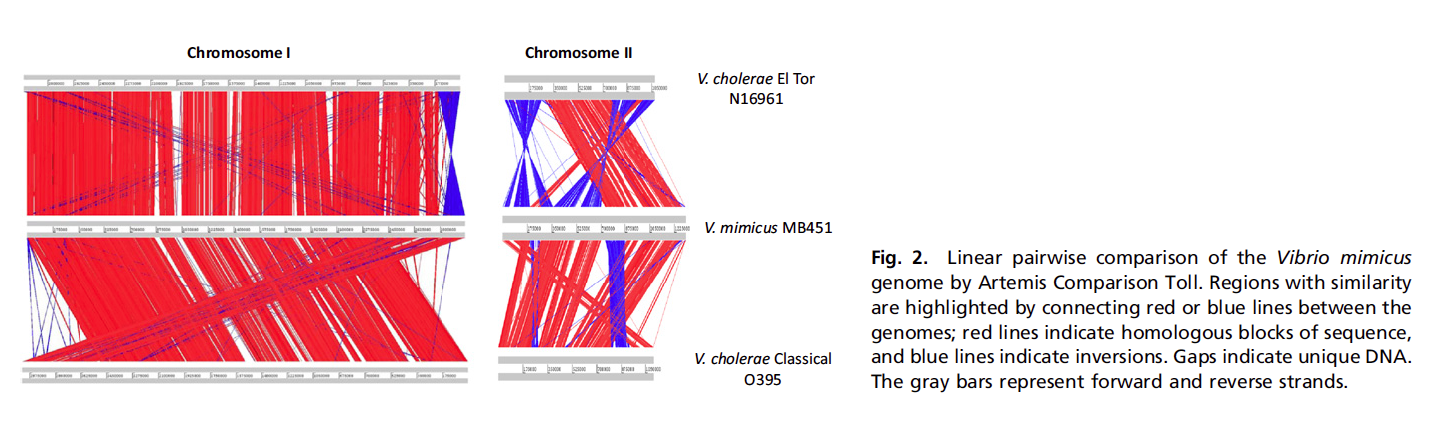
\includegraphics[width=1\textwidth]{images/v_mimicus}
  \end{center}    
  Suggests modularity of genome organisation, as a mechanism for adaptation (HGT, two-speed genome).
\end{frame}

% Serratia symbiotica
\begin{frame}
  \frametitle{\textit{Serratia symbiotica} 
  \footnote{\tiny{\href{http://dx.doi.org/10.1093/gbe/evr002}{Burke and Moran (2011) \textit{Genome Biol. Evol.} \textbf{3}:195-208 doi:10.1093/gbe/evr002}}}
  }
  \textit{S. symbiotica} is a recently evolved symbiont of aphids\\
  \textcolor{hutton_purple}{Massive genomic decay is an adaptation to the new environment.}\\
  \begin{center}
    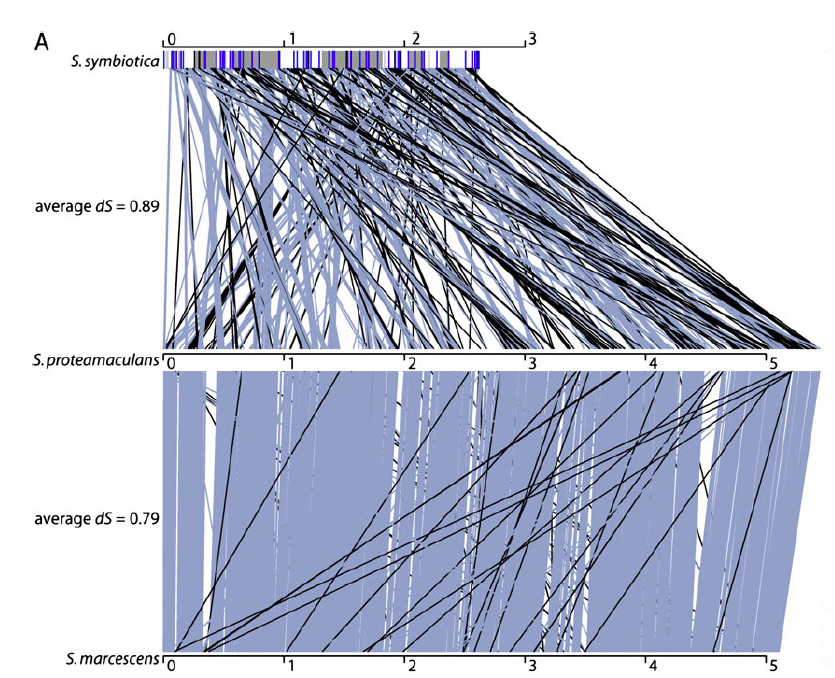
\includegraphics[width=0.75\textheight]{images/s_symbiotica}
  \end{center}    
\end{frame}

%
\begin{frame}
  \frametitle{Multiple genome alignments}
  \textcolor{olive}{Multiple genome alignments are ``harder'' than pairwise} \\
  \begin{itemize}
    \item Computationally difficult to produce
    \item \textcolor{red}{Lead to NP-complete optimisation problems!}
  \end{itemize}  
  \textcolor{hutton_green}{Solutions:} \textbf{heuristics}
  \begin{itemize}
    \item Progressive (build a tree, combine pairwise alignments)
    \item Iterative (realign initial sequences as new genomes added)
    \item \textcolor{hutton_blue}{Positional homology}
    \item \textcolor{hutton_purple}{\textit{Glocal} alignments}
  \end{itemize}  
\end{frame}

%
\begin{frame}
  \frametitle{Multiple genome alignment}
  Many tools either positional homology or glocal alignment
  \begin{columns}[T] 
    \column{.5\textwidth} 
      \textcolor{olive}{Several tools:}
      \begin{itemize}
        \item Mugsy: {\tiny\href{http://mugsy.sourceforge.net/}{(http://mugsy.sourceforge.net/)}}
        \item \textcolor{hutton_blue}{MLAGAN: {\tiny\href{http://lagan.stanford.edu/lagan_web/index.shtml}{(http://lagan.stanford.edu/lagan\_web/index.shtml)}}}
        \item TBA/MultiZ: {\tiny\href{http://www.bx.psu.edu/miller_lab/}{(http://www.bx.psu.edu/miller\_lab/)}}
        \item \textcolor{red}{\textbf{Mauve}: {\tiny\href{http://gel.ahabs.wisc.edu/mauve/}{(http://gel.ahabs.wisc.edu/mauve/)}}}
      \end{itemize}
    \column{.5\textwidth}
      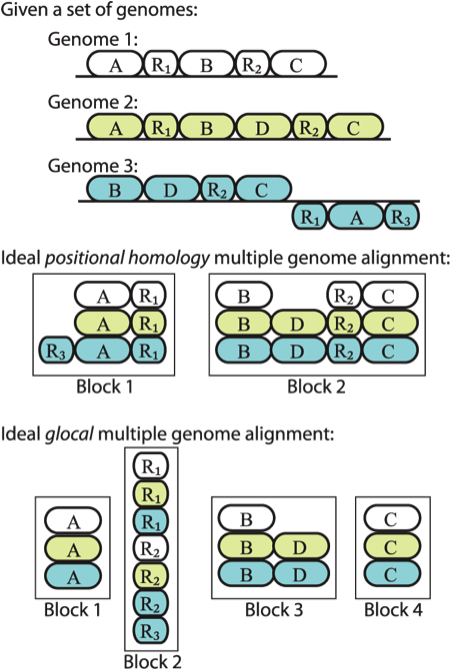
\includegraphics[width=0.75\textwidth]{images/poshom_v_glocal}
  \end{columns}    
\end{frame}

%
\begin{frame}
  \frametitle{MAUVE
  \footnote{\tiny{\href{http://dx.doi.org/10.1101/gr.2289704
}{Darling \textit{et al.} (2003) \textit{Genome Res.} doi:10.1101/gr.2289704
}}}
  }
  MAUVE/Progressive MAUVE: \href{http://gel.ahabs.wisc.edu/mauve/}{http://gel.ahabs.wisc.edu/mauve/} \\
  \begin{columns}[T] 
    \column{.55\textwidth} 
      \textcolor{RawSienna}{Algorithm:}
      \begin{enumerate}
        \item \textcolor{hutton_green}{Find local alignments (\textit{multi-MUMs}, A)}
        \item Build guide tree from multi-MUMs
        \item \textcolor{hutton_blue}{Select subset of multi-MUMs (\textit{anchors}, B)}
        \begin{itemize}
          \item Partition into \textit{local collinear blocks} (LCBs)
        \end{itemize}
        \item \textcolor{hutton_purple}{Recursive anchoring to refine anchors (C)}
        \item Progressive alignment against guide tree
      \end{enumerate}
    \column{.45\textwidth}
      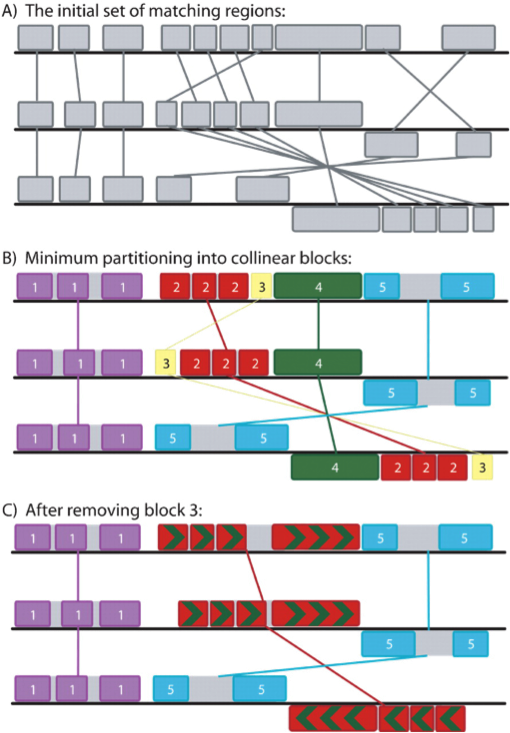
\includegraphics[width=0.9\textwidth]{images/mauve_method}
  \end{columns}    
\end{frame}

%
\begin{frame}
  \frametitle{MAUVE
  \footnote{\tiny{\href{http://dx.doi.org/10.1101/gr.2289704
}{Darling \textit{et al.} (2003) \textit{Genome Res.} doi:10.1101/gr.2289704
}}}
  }
  MAUVE alignment of LCBs in nine enterobacterial genomes \\
  \textcolor{hutton_green}{Evidence for rearrangement of homologous backbone sequence}
  \begin{center}
    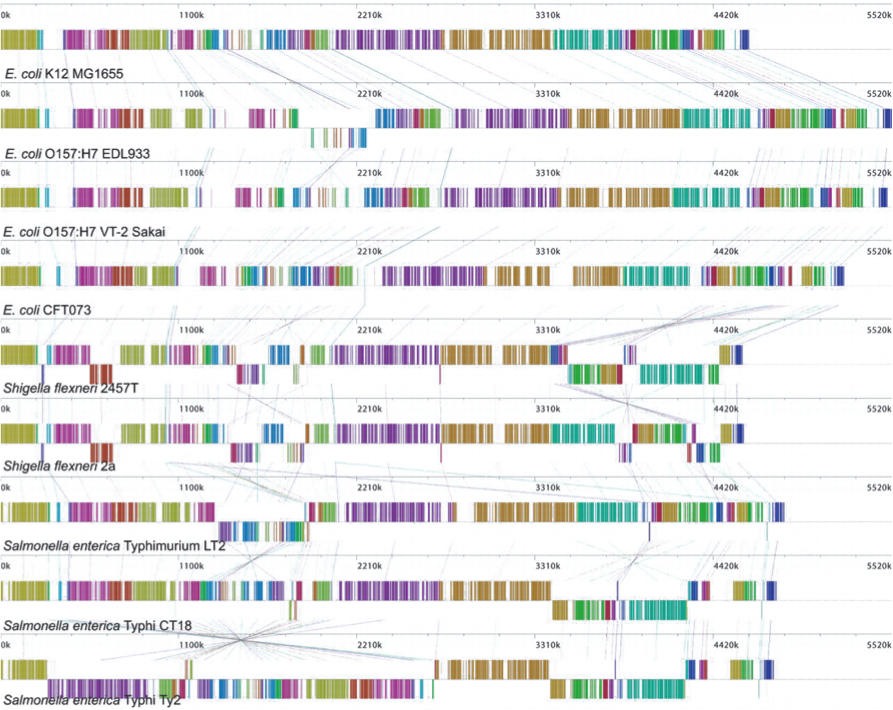
\includegraphics[height=0.6\textheight]{images/mauve_entero}
  \end{center}    
\end{frame}

%
\begin{frame}
  \frametitle{Draft genome alignment}
  \textcolor{olive}{High-throughput genome assemblies may be fragments (contigs)} \\
  Contigs can be ordered (\textit{scaffolded}):
  \begin{itemize}
    \item \textcolor{hutton_blue}{without alignment}, by long or paired-end reads
    \item \textcolor{hutton_purple}{by alignment}, to complete \textit{reference} genomes
    \item \textcolor{hutton_purple}{by alignment}, to other draft incomplete genomes
  \end{itemize}
  \begin{center}
    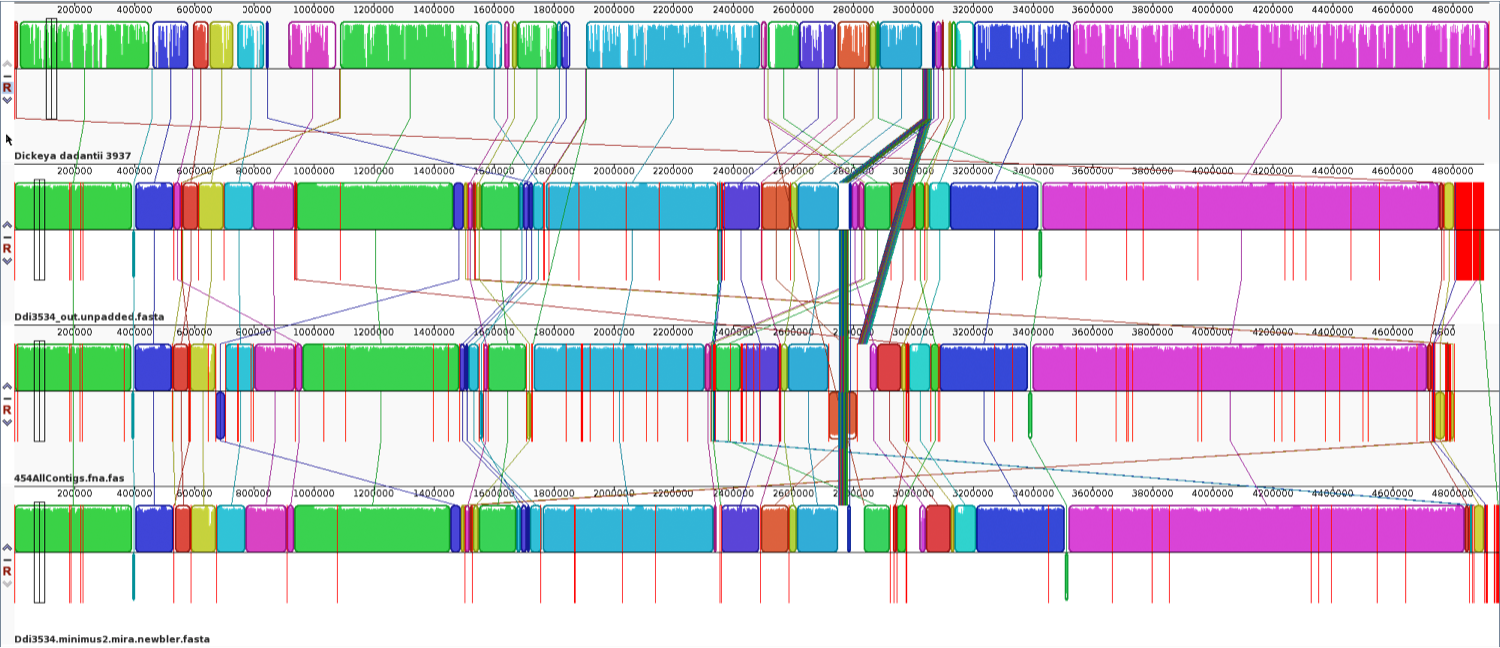
\includegraphics[width=\textwidth]{images/mauve_scaffolding}
  \end{center}    
\end{frame}

% DNA-DNA hybridisation
\begin{frame}
  \frametitle{Chromosome painting\footnote{\tiny{\href{http://dx.doi.org/10.1093/molbev/mst055}{Yahara \textit{et al}. (2013) \textit{Mol. Biol. Evol.} \textbf{30}:1454-1464 doi:10.1093/molbev/mst055}}}}
  ``Chromosome painting'' infers recombination-derived `chunks'\\
  Genome's haplotype constructed in terms of recombination events from a `donor' to a `recipient' genome\\
  \begin{center}
    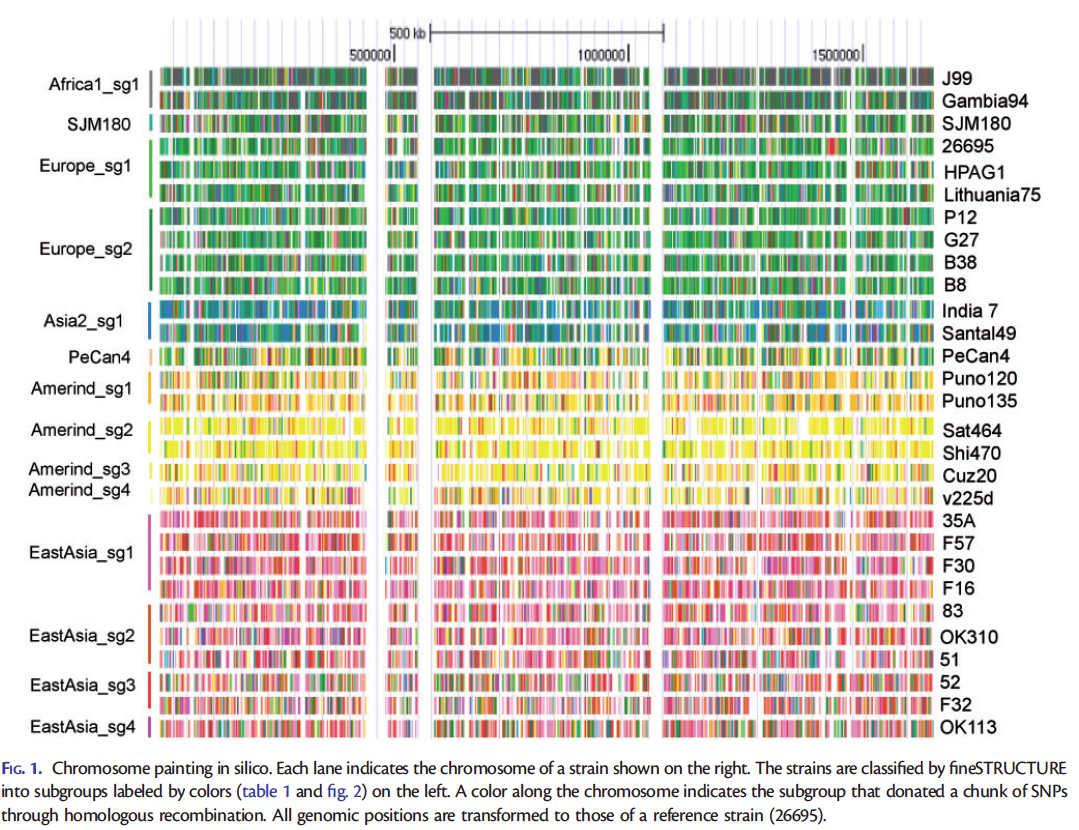
\includegraphics[width=0.7\textwidth]{images/chromosome_painting}
  \end{center}     
\end{frame}

% DNA-DNA hybridisation
\begin{frame}
  \frametitle{Chromosome painting\footnote{\tiny{\href{http://dx.doi.org/10.1093/molbev/mst055}{Yahara \textit{et al}. (2013) \textit{Mol. Biol. Evol.} \textbf{30}:1454-1464 doi:10.1093/molbev/mst055}}}}
  Recombination events summarised in a \textit{coancestry matrix}.\\
  \textit{H. pylori}: most within geographical bounds, but asymmetrical donation from Amerind/East Asian to European isolates.
  \begin{center}
    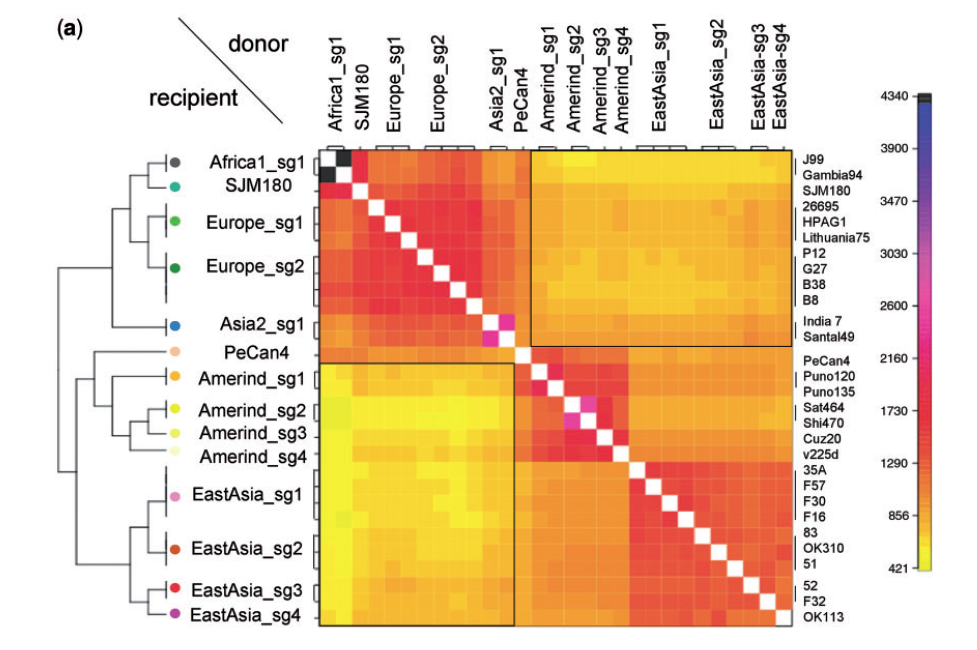
\includegraphics[width=0.75\textwidth]{images/coancestry}
  \end{center}     
\end{frame}

%
\begin{frame}
  \frametitle{Whole Genome Comparisons}
  \textcolor{RawSienna}{Physical and computational genome comparisons} \\
  \begin{itemize}
    \item Similar biological questions
    \item \textcolor{red}{$\therefore$ similar concepts}
  \end{itemize}  
  \textcolor{hutton_green}{Modern biology: lots of sequence data}
  \begin{itemize}
    \item Conservation $\approx$ evolutionary constraint
    \item \textcolor{hutton_blue}{Many choices of algorithms/software}
    \item \textcolor{hutton_purple}{Many choices of visualisation tools/software}
  \end{itemize}  
\end{frame}
